\begin{equation}
\Pggx(q) + \Pg(k_1) \rightarrow \PaQ(p_2) + \PQ(p_1) + \Pg(k_2)
\end{equation}

diagramatic:
\begin{figure}[ht!]
	\centering
	\begin{subfigure}[t]{.4\textwidth}
		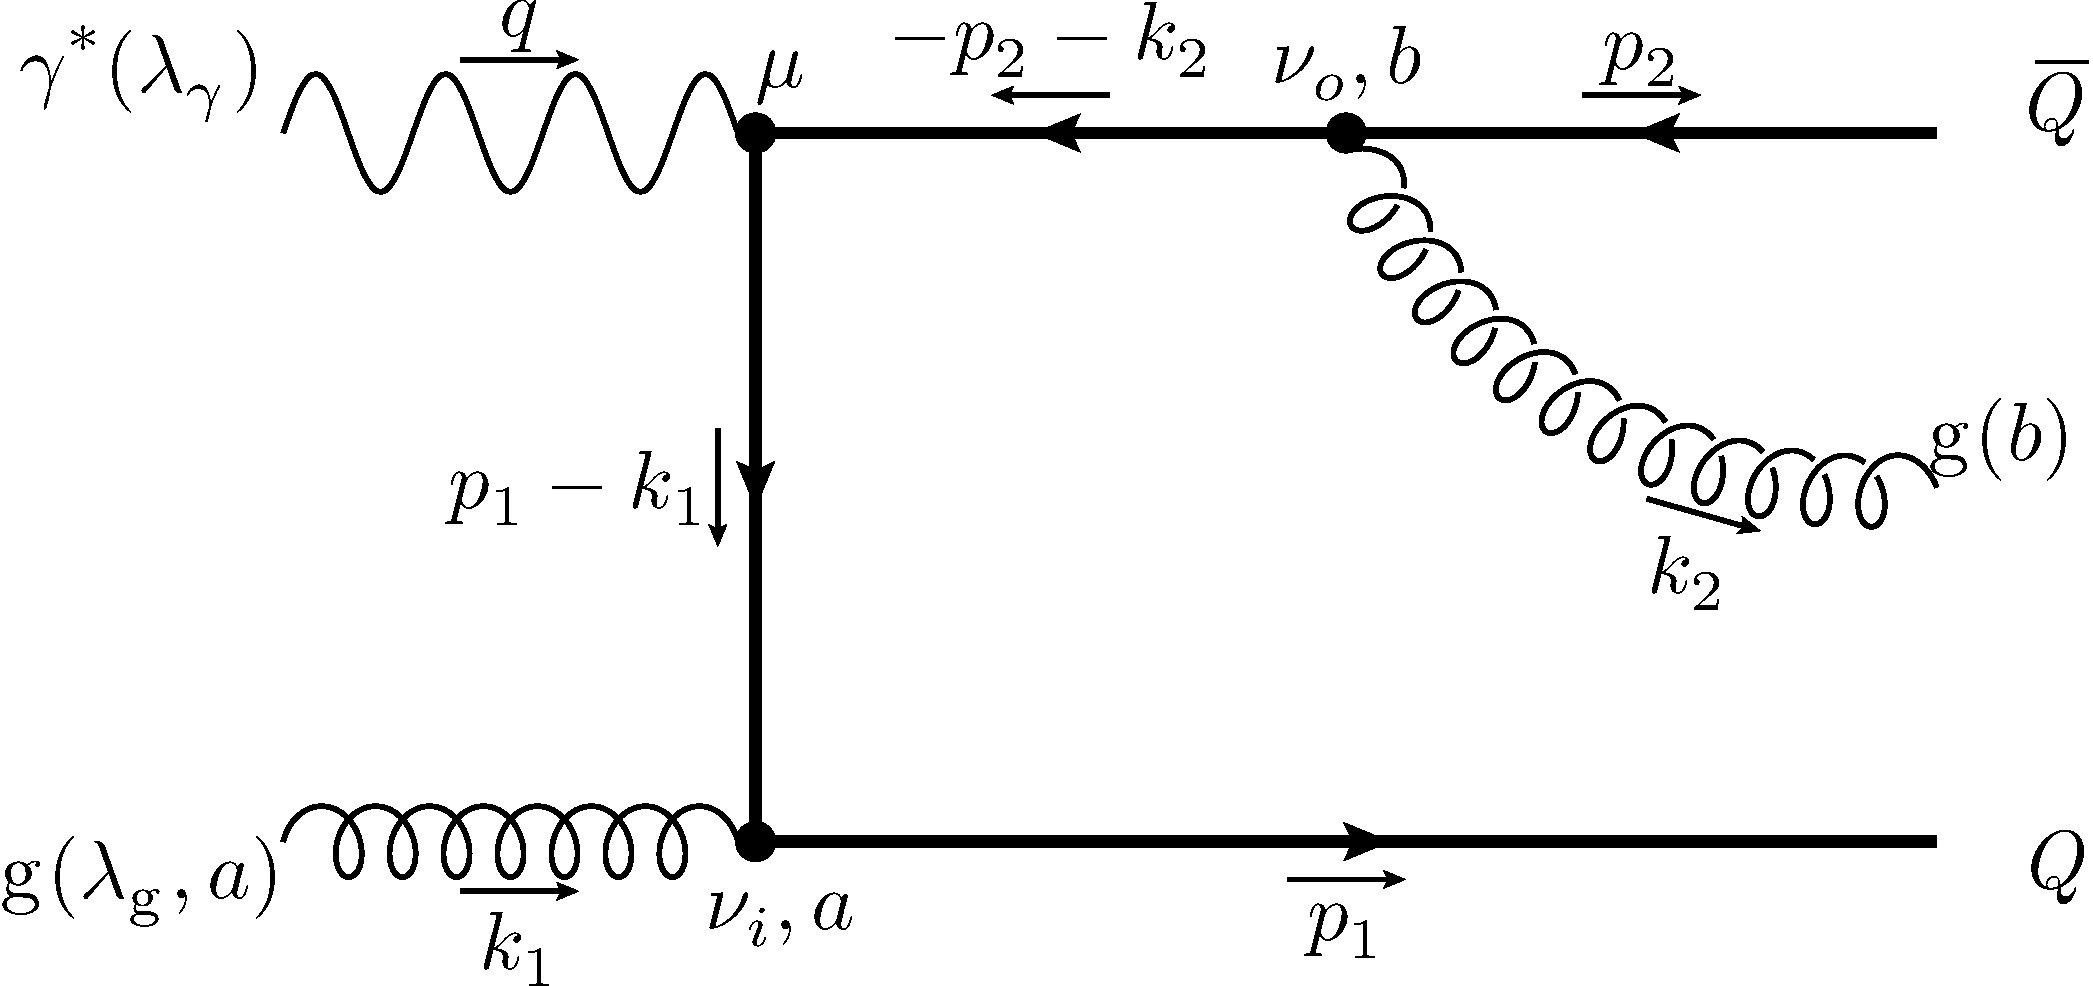
\includegraphics[width=\textwidth]{pyfeyn/nlo-g-1}
		\caption{$i\Md^{(NLO,g)}_{1,\mu}$}
	\end{subfigure}\hspace{.15\textwidth}%
	\begin{subfigure}[t]{.4\textwidth}
		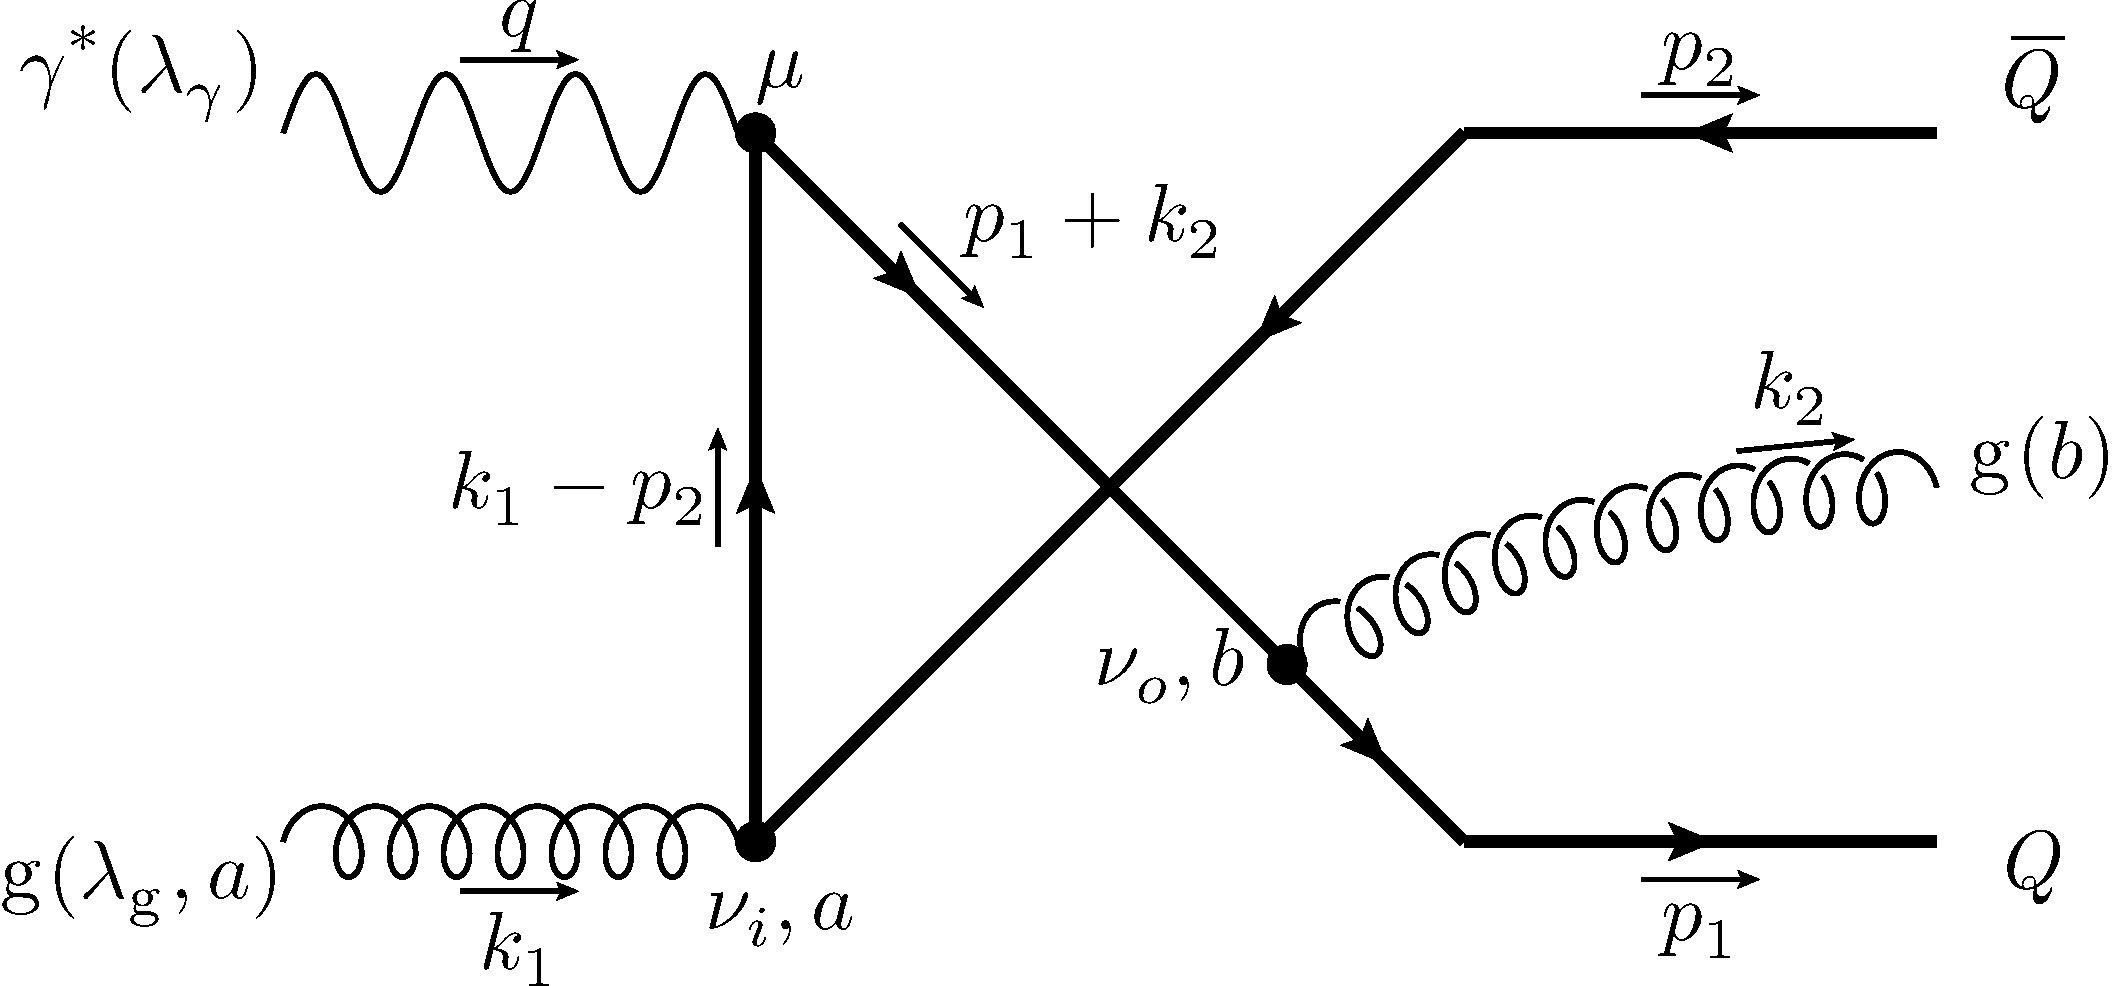
\includegraphics[width=\textwidth]{pyfeyn/nlo-g-2}
		\caption{$i\Md^{(NLO,g)}_{2,\mu}$}
	\end{subfigure}\\
	\begin{subfigure}[t]{.42\textwidth}
		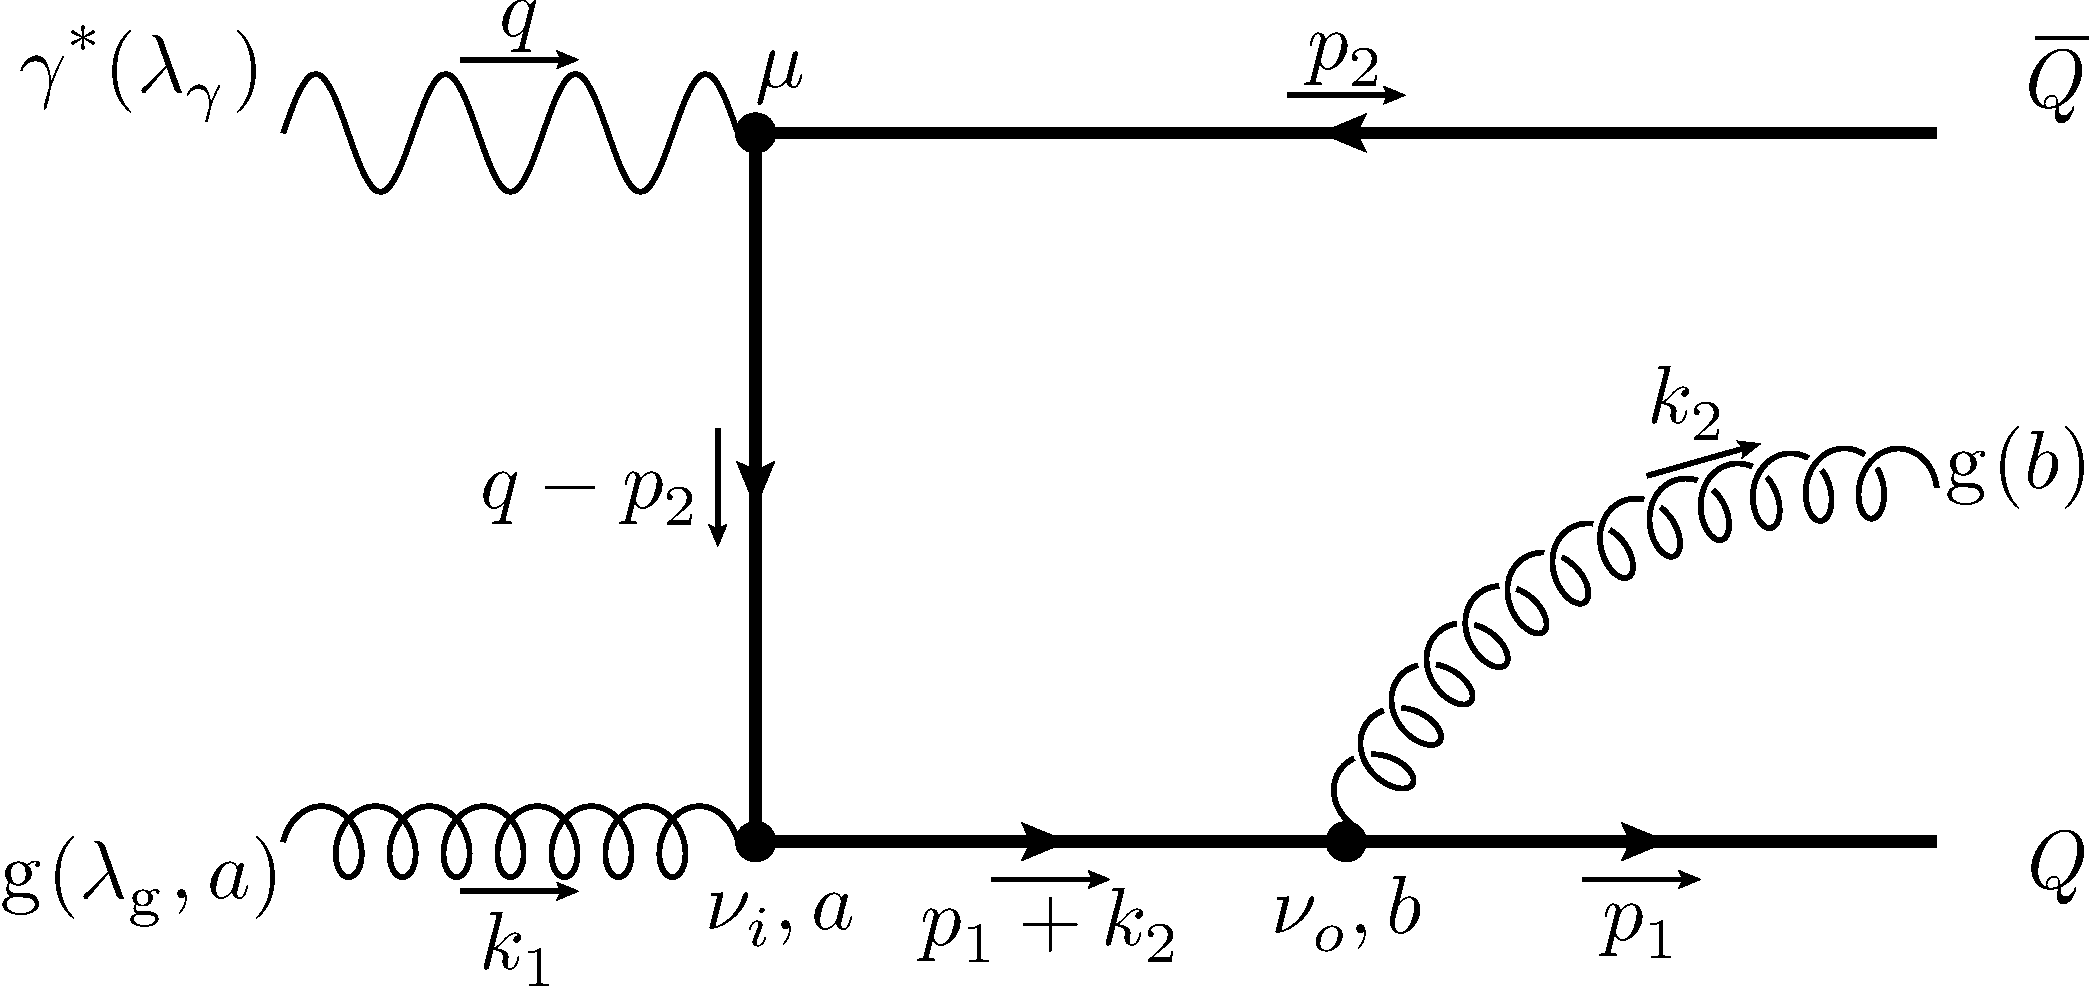
\includegraphics[width=\textwidth]{pyfeyn/nlo-g-3}
		\caption{$i\Md^{(NLO,g)}_{3,\mu}$}
	\end{subfigure}\hspace{.1\textwidth}%
	\begin{subfigure}[t]{.42\textwidth}
		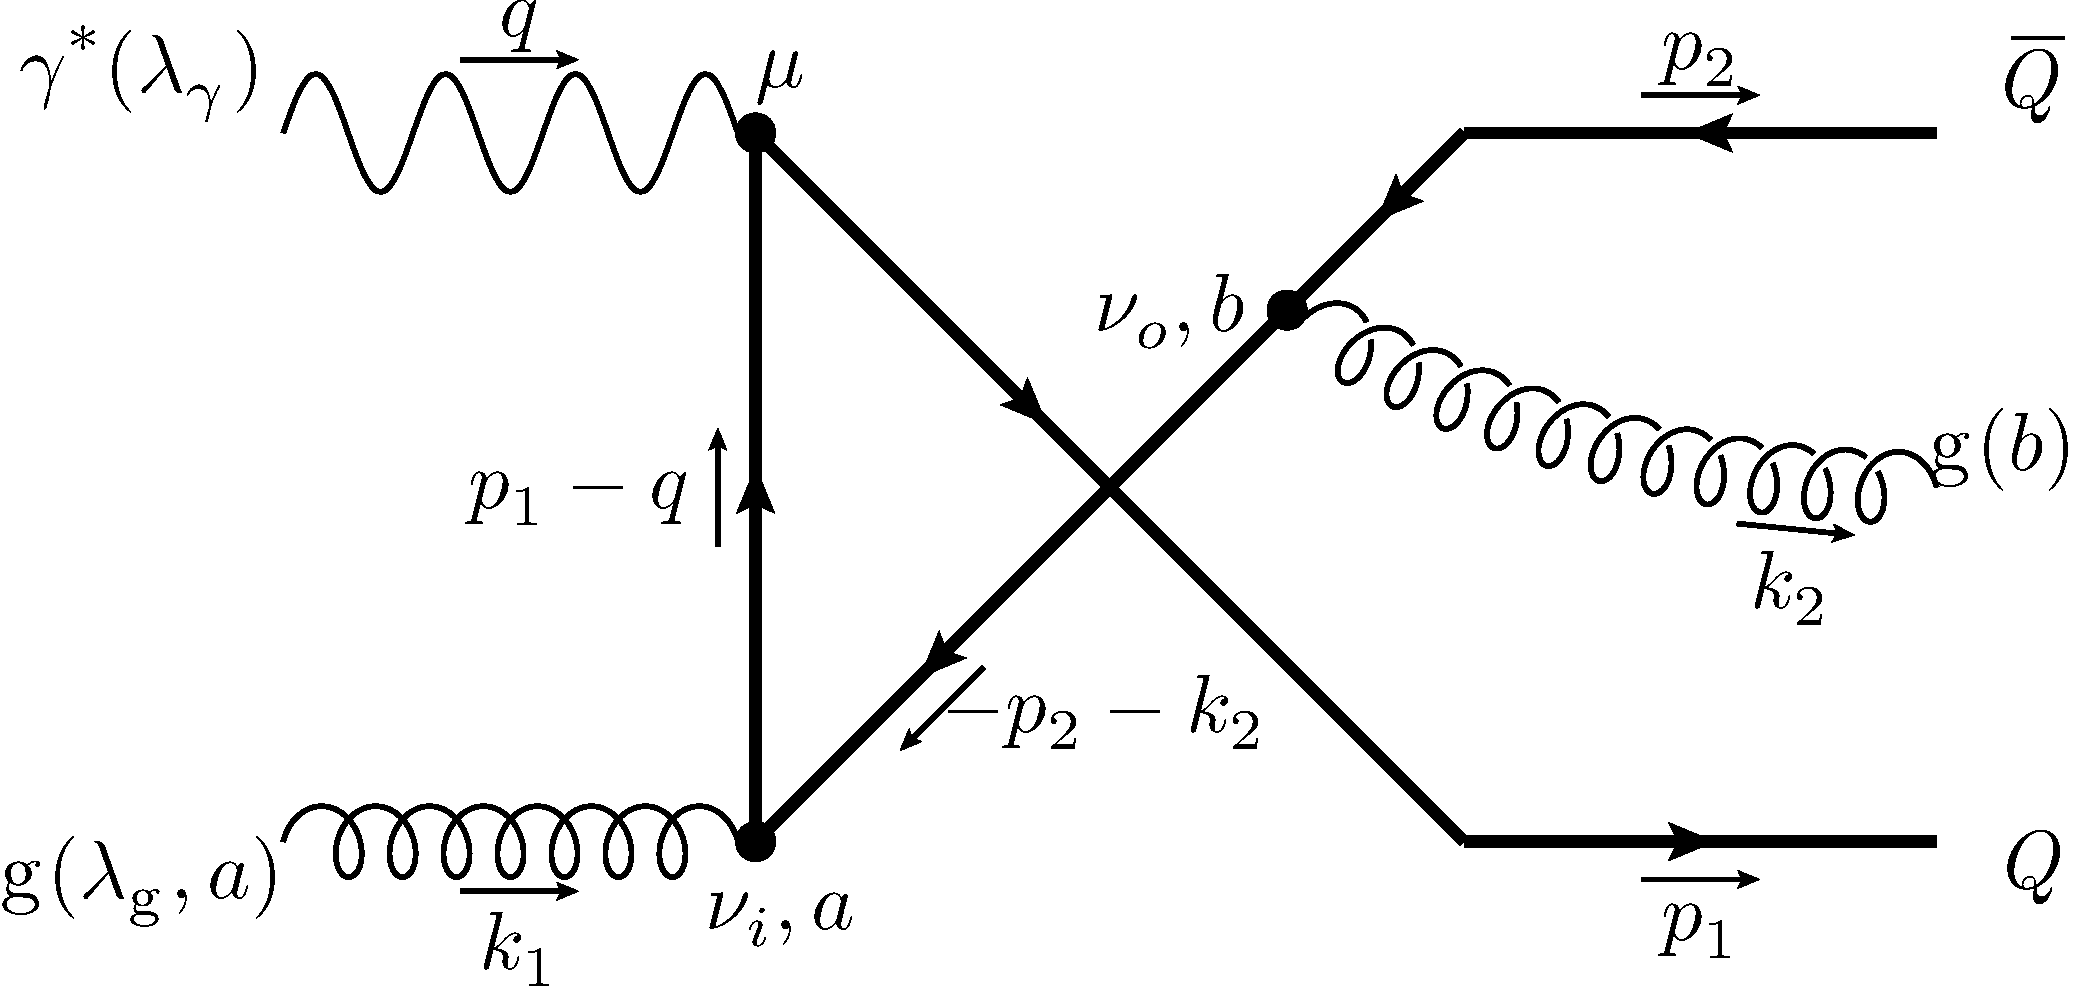
\includegraphics[width=\textwidth]{pyfeyn/nlo-g-4}
		\caption{$i\Md^{(NLO,g)}_{4,\mu}$}
	\end{subfigure}\\
	\begin{subfigure}[t]{.4\textwidth}
		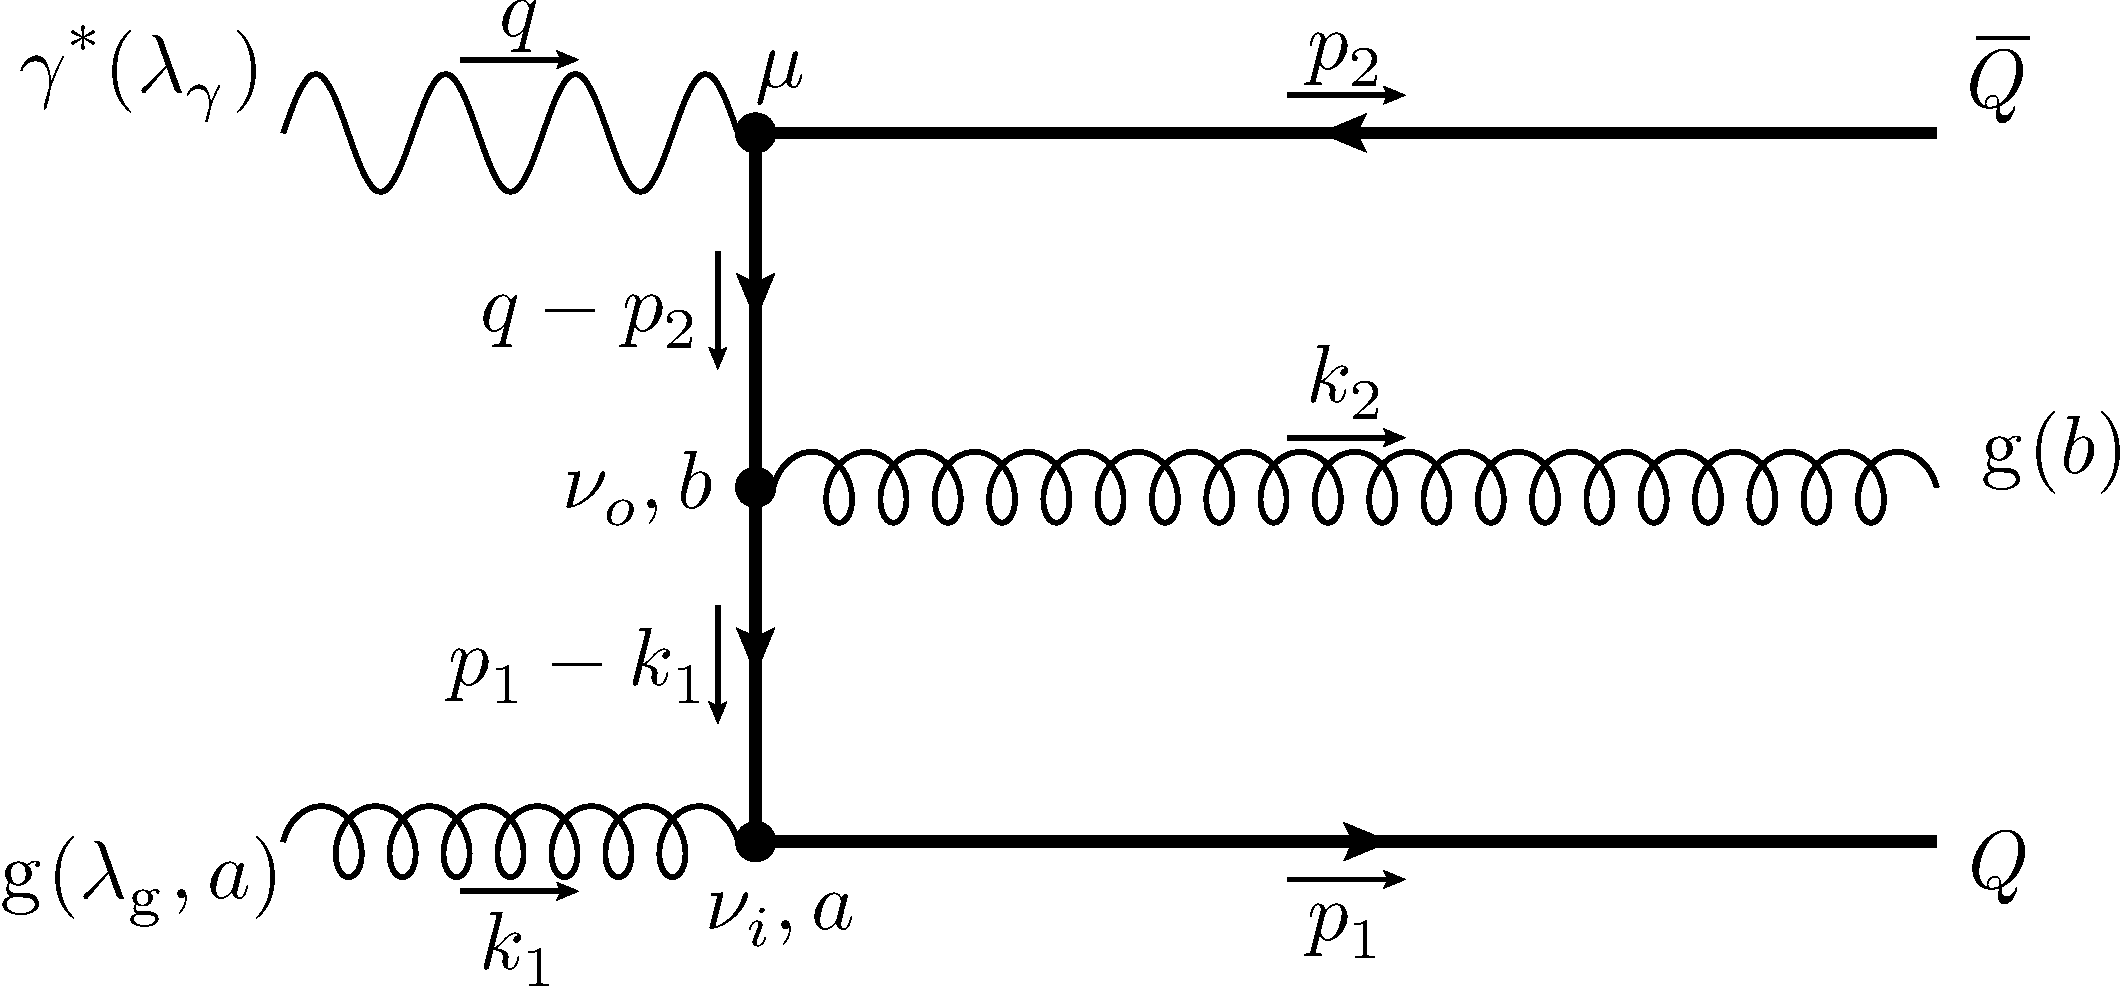
\includegraphics[width=\textwidth]{pyfeyn/nlo-g-5}
		\caption{$i\Md^{(NLO,g)}_{5,\mu}$}
	\end{subfigure}\hspace{.15\textwidth}%
	\begin{subfigure}[t]{.4\textwidth}
		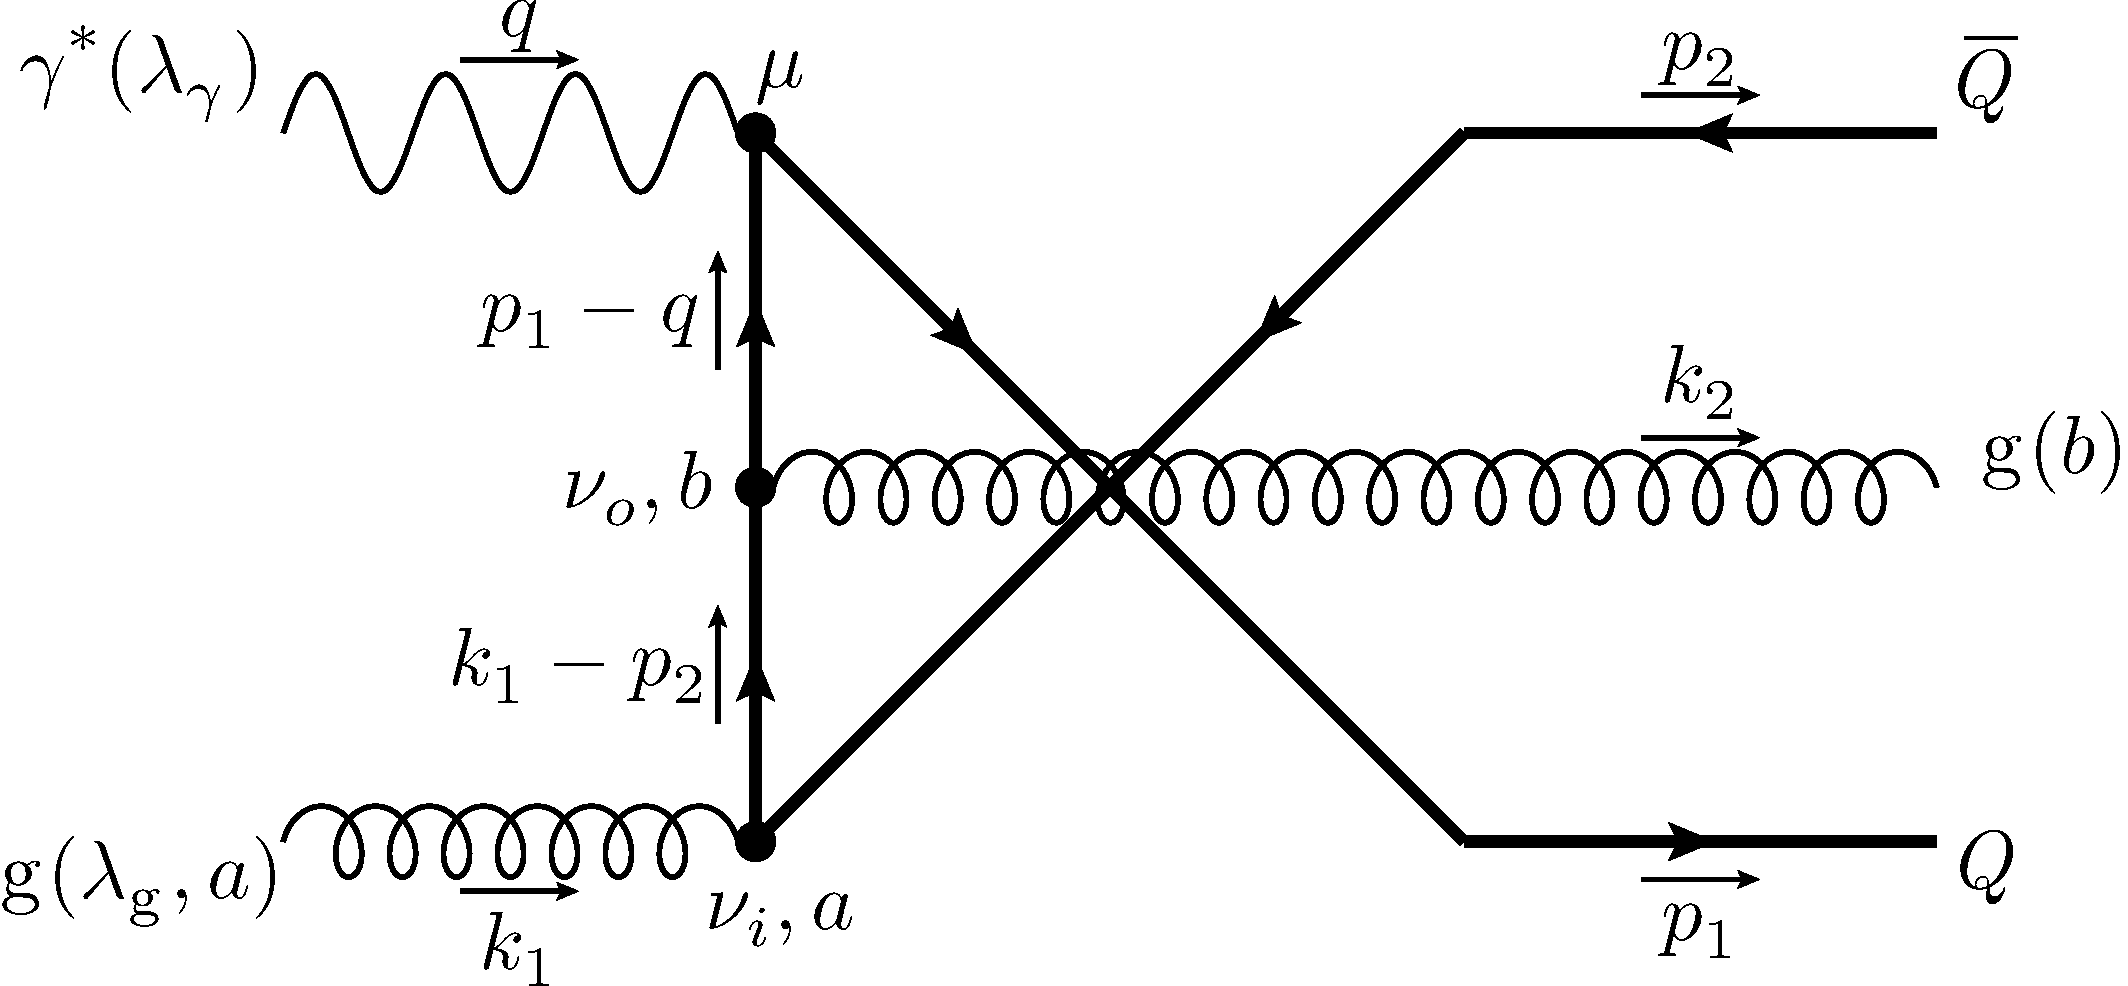
\includegraphics[width=\textwidth]{pyfeyn/nlo-g-6}
		\caption{$i\Md^{(NLO,g)}_{6,\mu}$}
	\end{subfigure}\\
	\begin{subfigure}[t]{.42\textwidth}
		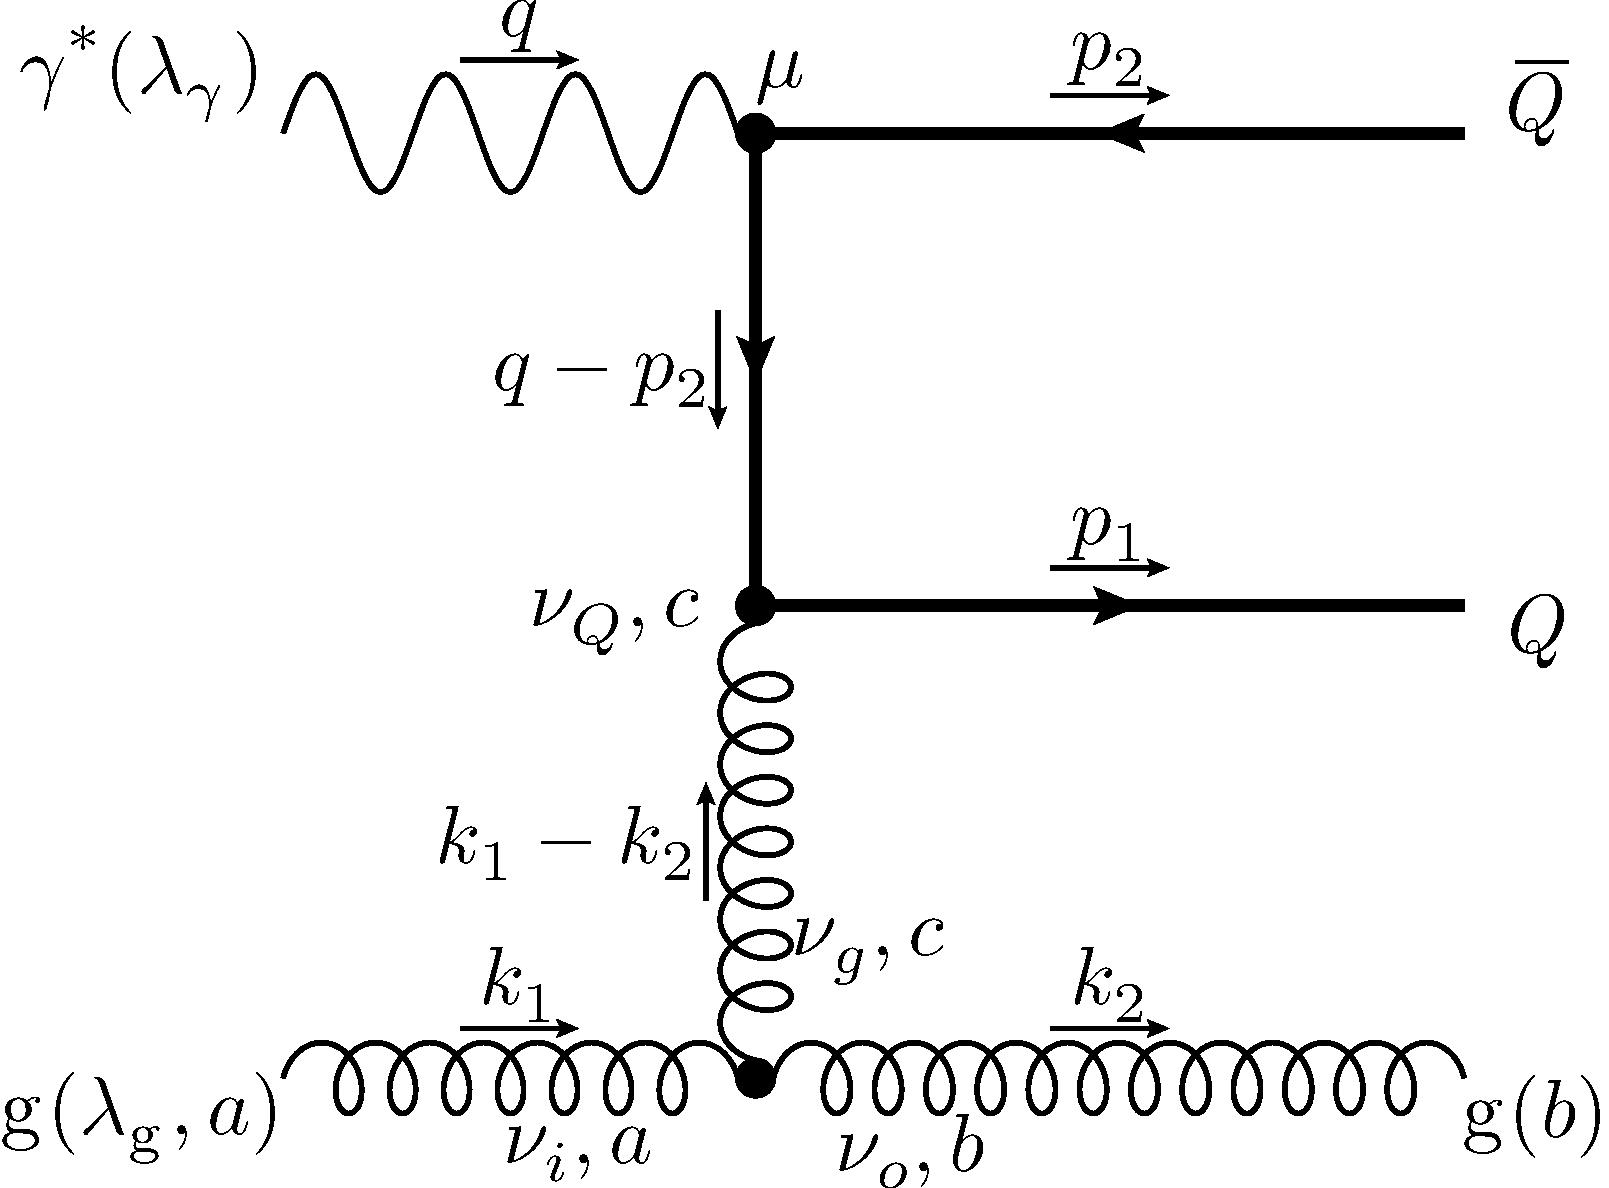
\includegraphics[width=\textwidth]{pyfeyn/nlo-g-7}
		\caption{$i\Md^{(NLO,g)}_{7,\mu}$}
	\end{subfigure}\hspace{.1\textwidth}%
	\begin{subfigure}[t]{.42\textwidth}
		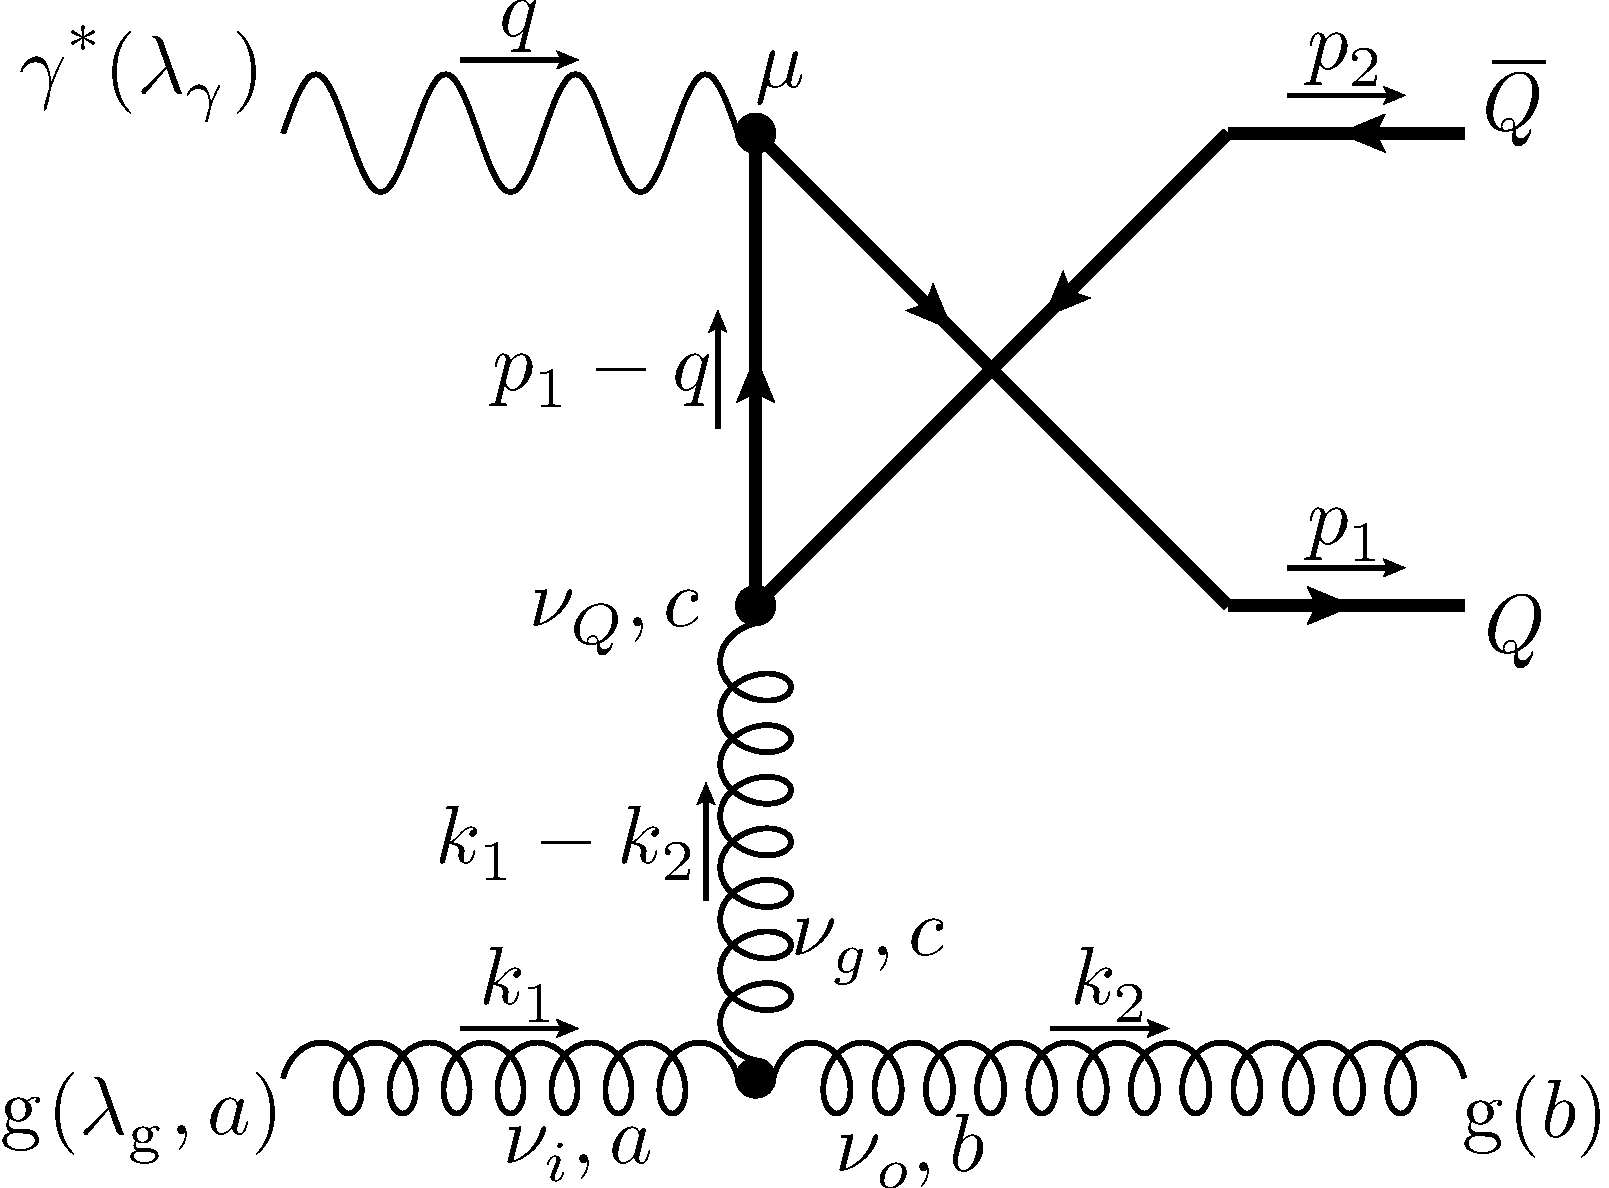
\includegraphics[width=\textwidth]{pyfeyn/nlo-g-8}
		\caption{$i\Md^{(NLO,g)}_{8,\mu}$}
	\end{subfigure}
	\caption{NLO contributions by gluon bremsstrahlung}\label{fig:FeynNLOg}
\end{figure}

formula:
\begin{align}
i\Md^{(NLO,g)}_{1,\mu} &= \bar u(p_1)(igT_a\gamma^{\nu_i})\frac{i(\slashed{p}_1-\slashed{k}_1+m)}{u_6}(-i e e_H \gamma_\mu)\cdot\nonumber\\
 &\hspace{40pt}\frac{i(-\slashed{p}_2-\slashed{k}_2+m)}{s_3}(igT_b\gamma^{\nu_o})v(p_2)\varepsilon^{(\lambda_{\Pg})}_{\nu_i}(k_1)\varepsilon_{\nu_o}(k_2)\\
i\Md^{(NLO,g)}_{2,\mu} &= \bar u(p_1)(igT_b\gamma^{\nu_o})\frac{i(\slashed{p}_1+\slashed{k}_2+m)}{s_4}(-i e e_H \gamma_\mu)\cdot\nonumber\\
 &\hspace{40pt}\frac{i(\slashed{k}_1-\slashed{p}_2+m)}{t_1}(igT_a\gamma^{\nu_i})v(p_2)\varepsilon^{(\lambda_{\Pg})}_{\nu_i}(k_1)\varepsilon_{\nu_o}(k_2)\\
i\Md^{(NLO,g)}_{3,\mu} &= \bar u(p_1)(igT_b\gamma^{\nu_o})\frac{i(\slashed{p}_1+\slashed{k}_2+m)}{s_4}(igT_a\gamma^{\nu_i})\cdot\nonumber\\
 &\hspace{40pt}\frac{i(\slashed{q}-\slashed{p}_2+m)}{u_1}(-i e e_H \gamma_\mu)v(p_2)\varepsilon^{(\lambda_{\Pg})}_{\nu_i}(k_1)\varepsilon_{\nu_o}(k_2)\\
i\Md^{(NLO,g)}_{4,\mu} &= \bar u(p_1)(-i e e_H \gamma_\mu)\frac{i(\slashed{p}_1-\slashed{q}+m)}{u_7}(igT_a\gamma^{\nu_i})\cdot\nonumber\\
 &\hspace{40pt}\frac{i(-\slashed{p}_2-\slashed{k}_2+m)}{s_3}(igT_b\gamma^{\nu_o})v(p_2)\varepsilon^{(\lambda_{\Pg})}_{\nu_i}(k_1)\varepsilon_{\nu_o}(k_2)\\
i\Md^{(NLO,g)}_{5,\mu} &= \bar u(p_1)(igT_a\gamma^{\nu_i})\frac{i(\slashed{p}_1-\slashed{k}_1+m)}{u_6}(igT_b\gamma^{\nu_o})\cdot\nonumber\\
 &\hspace{40pt}\frac{i(\slashed{q}-\slashed{p}_2+m)}{u_1}(-i e e_H \gamma_\mu)v(p_2)\varepsilon^{(\lambda_{\Pg})}_{\nu_i}(k_1)\varepsilon_{\nu_o}(k_2)\\
i\Md^{(NLO,g)}_{6,\mu} &= \bar u(p_1)(-i e e_H \gamma_\mu)\frac{i(\slashed{p}_1-\slashed{q}+m)}{u_7}(igT_b\gamma^{\nu_o})\cdot\nonumber\\
 &\hspace{40pt}\frac{i(\slashed{k}_1-\slashed{p}_2+m)}{t_1}(igT_a\gamma^{\nu_i})v(p_2)\varepsilon^{(\lambda_{\Pg})}_{\nu_i}(k_1)\varepsilon_{\nu_o}(k_2)\\
i\Md^{(NLO,g)}_{7,\mu} &= \bar u(p_1)(igT_c\gamma^{\nu_Q})\frac{i(\slashed{q}-\slashed{p}_2+m)}{u_1}(-i e e_H \gamma_\mu)v(p_2)\cdot\frac{-ig_{\nu_Q,\nu_g}}{t'}\cdot\varepsilon^{(\lambda_{\Pg})}_{\nu_i}(k_1)\varepsilon_{\nu_o}(k_2)\cdot\nonumber\\
 &\hspace{30pt}\left(gf^{acb}\left(g^{\nu_o,\nu_i}(k_1+k_2)^{\nu_g}+g^{\nu_i,\nu_g}(k_2-2k_1)^{\nu_o}+g^{\nu_g,\nu_o}(k_1-2k_2)^{\nu_i}\right)\right)\\
i\Md^{(NLO,g)}_{8,\mu} &= \bar u(p_1)(-i e e_H \gamma_\mu)\frac{i(\slashed{p}_1-\slashed{q}+m)}{u_7}(igT_c\gamma^{\nu_Q})v(p_2)\cdot\frac{-ig_{\nu_Q,\nu_g}}{t'}\cdot\varepsilon^{(\lambda_{\Pg})}_{\nu_i}(k_1)\varepsilon_{\nu_o}(k_2)\cdot\nonumber\\
 &\hspace{30pt}\left(gf^{acb}\left(g^{\nu_o,\nu_i}(k_1+k_2)^{\nu_g}+g^{\nu_i,\nu_g}(k_2-2k_1)^{\nu_o}+g^{\nu_g,\nu_o}(k_1-2k_2)^{\nu_i}\right)\right)
\end{align}

color space:
\begin{align}
&\sum\limits_{j=1}^6\abs{\Md^{(NLO,g)}_{j,\mu}}^2 + \Md^{(NLO,g)}_{1,\mu}\left(\Md^{(NLO,g)}_{4,\mu'}+\Md^{(NLO,g)}_{5,\mu'}\right)^*+\Md^{(NLO,g)}_{3,\mu}\left(\Md^{(NLO,g)}_{6,\mu'}\right)^*+\nonumber\\
&\Md^{(NLO,g)}_{2,\mu}\left(\Md^{(NLO,g)}_{3,\mu'}+\Md^{(NLO,g)}_{6,\mu'}\right)^*+\Md^{(NLO,g)}_{4,\mu}\left(\Md^{(NLO,g)}_{5,\mu'}\right)^*\nonumber\\
&\sim\tr(T_aT_aT_bT_b) = N_C C_F^2\\
&\Md^{(NLO,g)}_{1,\mu}\left(\Md^{(NLO,g)}_{2,\mu'}+\Md^{(NLO,g)}_{3,\mu'}+\Md^{(NLO,g)}_{6,\mu'}\right)^*+\nonumber\\
&\left(\Md^{(NLO,g)}_{2,\mu}+\Md^{(NLO,g)}_{3,\mu}\right)\left(\Md^{(NLO,g)}_{4,\mu'}+\Md^{(NLO,g)}_{5,\mu'}\right)^*+\nonumber\\
&\left(\Md^{(NLO,g)}_{4,\mu}+\Md^{(NLO,g)}_{5,\mu}\right)\left(\Md^{(NLO,g)}_{6,\mu'}\right)^*\nonumber\\
&\sim\tr(T_aT_bT_aT_b) = N_C C_F \left(C_F - \frac{C_A}{2}\right)\\
&\left(\Md^{(NLO,g)}_{2,\mu}+\Md^{(NLO,g)}_{3,\mu}+\Md^{(NLO,g)}_{6,\mu}\right)\left(\Md^{(NLO,g)}_{7,\mu'}+\Md^{(NLO,g)}_{8,\mu'}\right)^*\nonumber\\
&\sim-if_{bda}\tr(T_aT_bT_d) = \frac 1 2 N_C C_F C_A\\
&\left(\Md^{(NLO,g)}_{1,\mu}+\Md^{(NLO,g)}_{4,\mu}+\Md^{(NLO,g)}_{5,\mu}\right)\left(\Md^{(NLO,g)}_{7,\mu'}+\Md^{(NLO,g)}_{8,\mu'}\right)^*\nonumber\\
&\sim-if_{bda}\tr(T_bT_aT_d) = if_{bda}\tr(T_aT_bT_d)=-\frac 1 2 N_C C_F C_A\\
&\abs{\Md^{(NLO,g)}_{7,\mu}+\Md^{(NLO,g)}_{8,\mu}}^2 \nonumber\\
&\sim f_{acb}f_{adb}\tr(T_cT_d) = N_C C_F C_A
\end{align}

\pagebreak
To get the polarisation sums right, one has to subtract the contributions of the Faddeev-Popov ghosts\cite{FADDEEV196729,QFT}:

diagramatic:
\begin{figure}[ht!]
	\centering
	\begin{subfigure}[t]{.4\textwidth}
		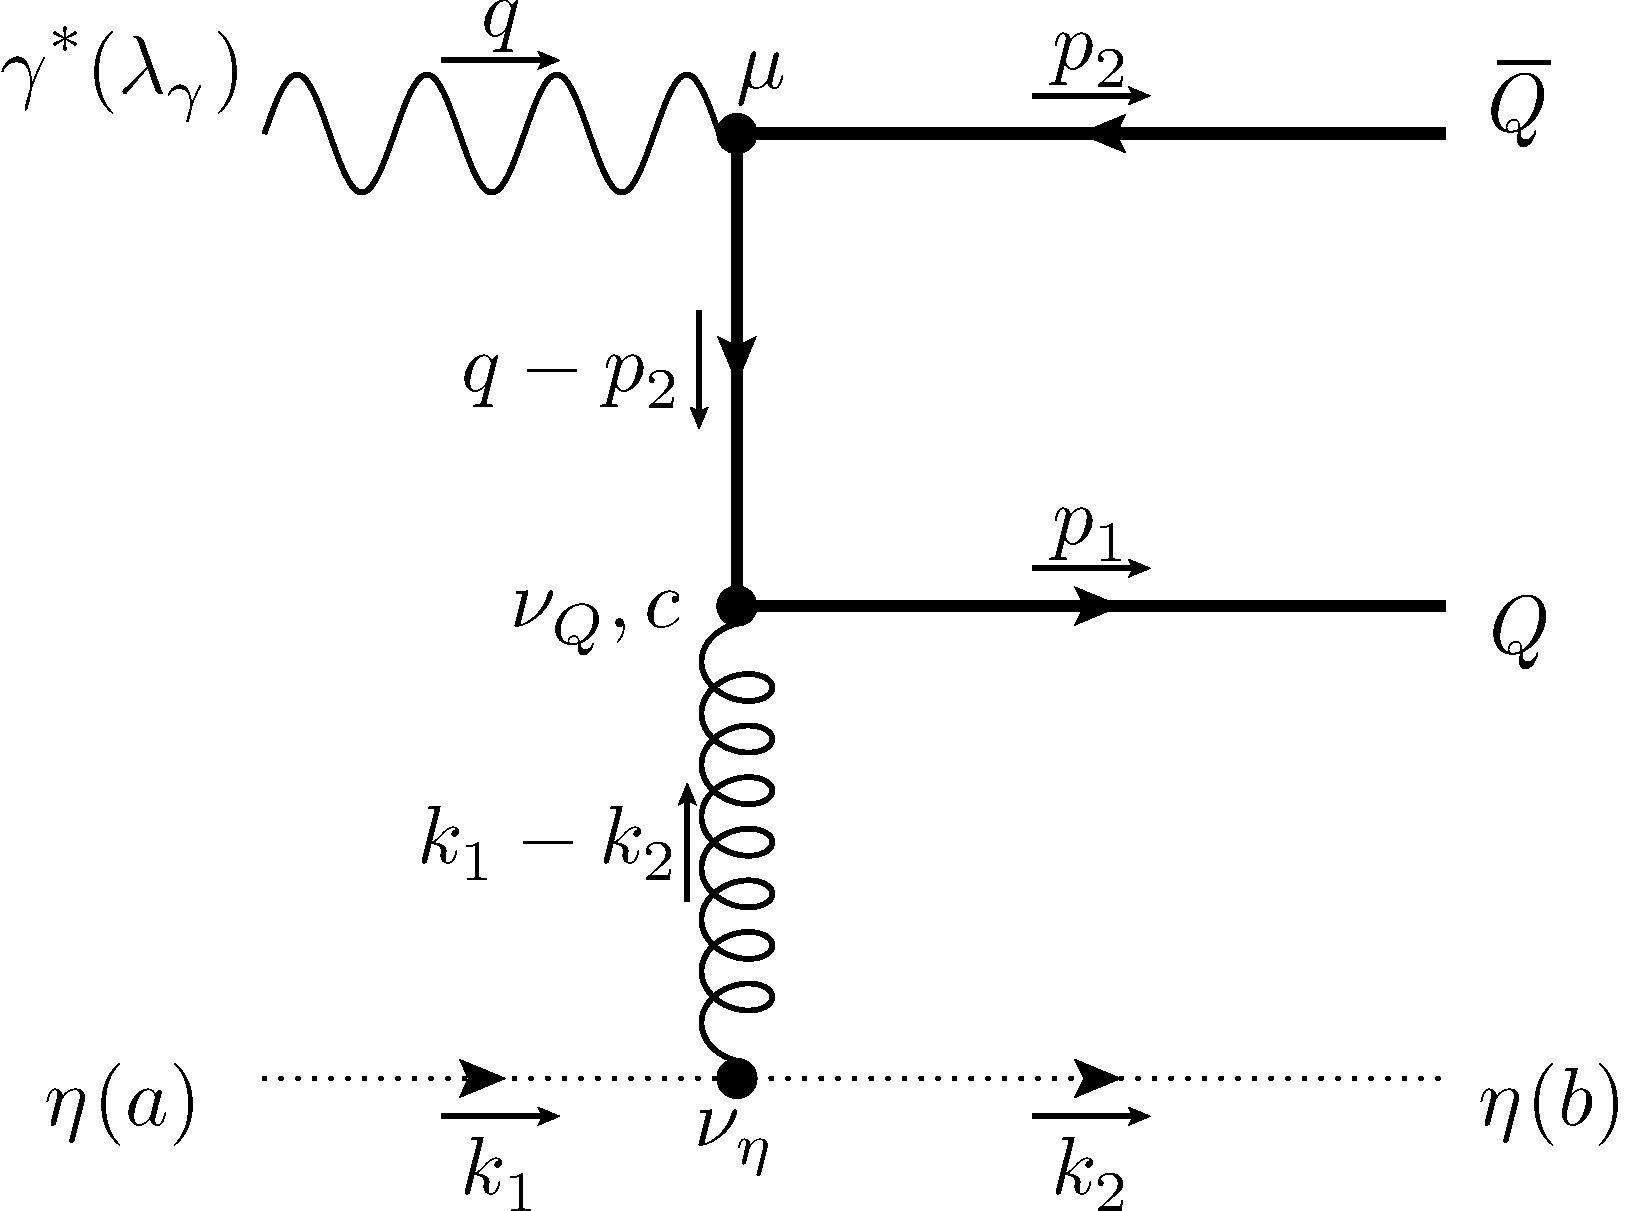
\includegraphics[width=\textwidth]{pyfeyn/nlo-gh-1}
		\caption{$i\Md^{(NLO,\Pgh)}_{1,\mu}$}
	\end{subfigure}\hspace{.15\textwidth}%
	\begin{subfigure}[t]{.4\textwidth}
		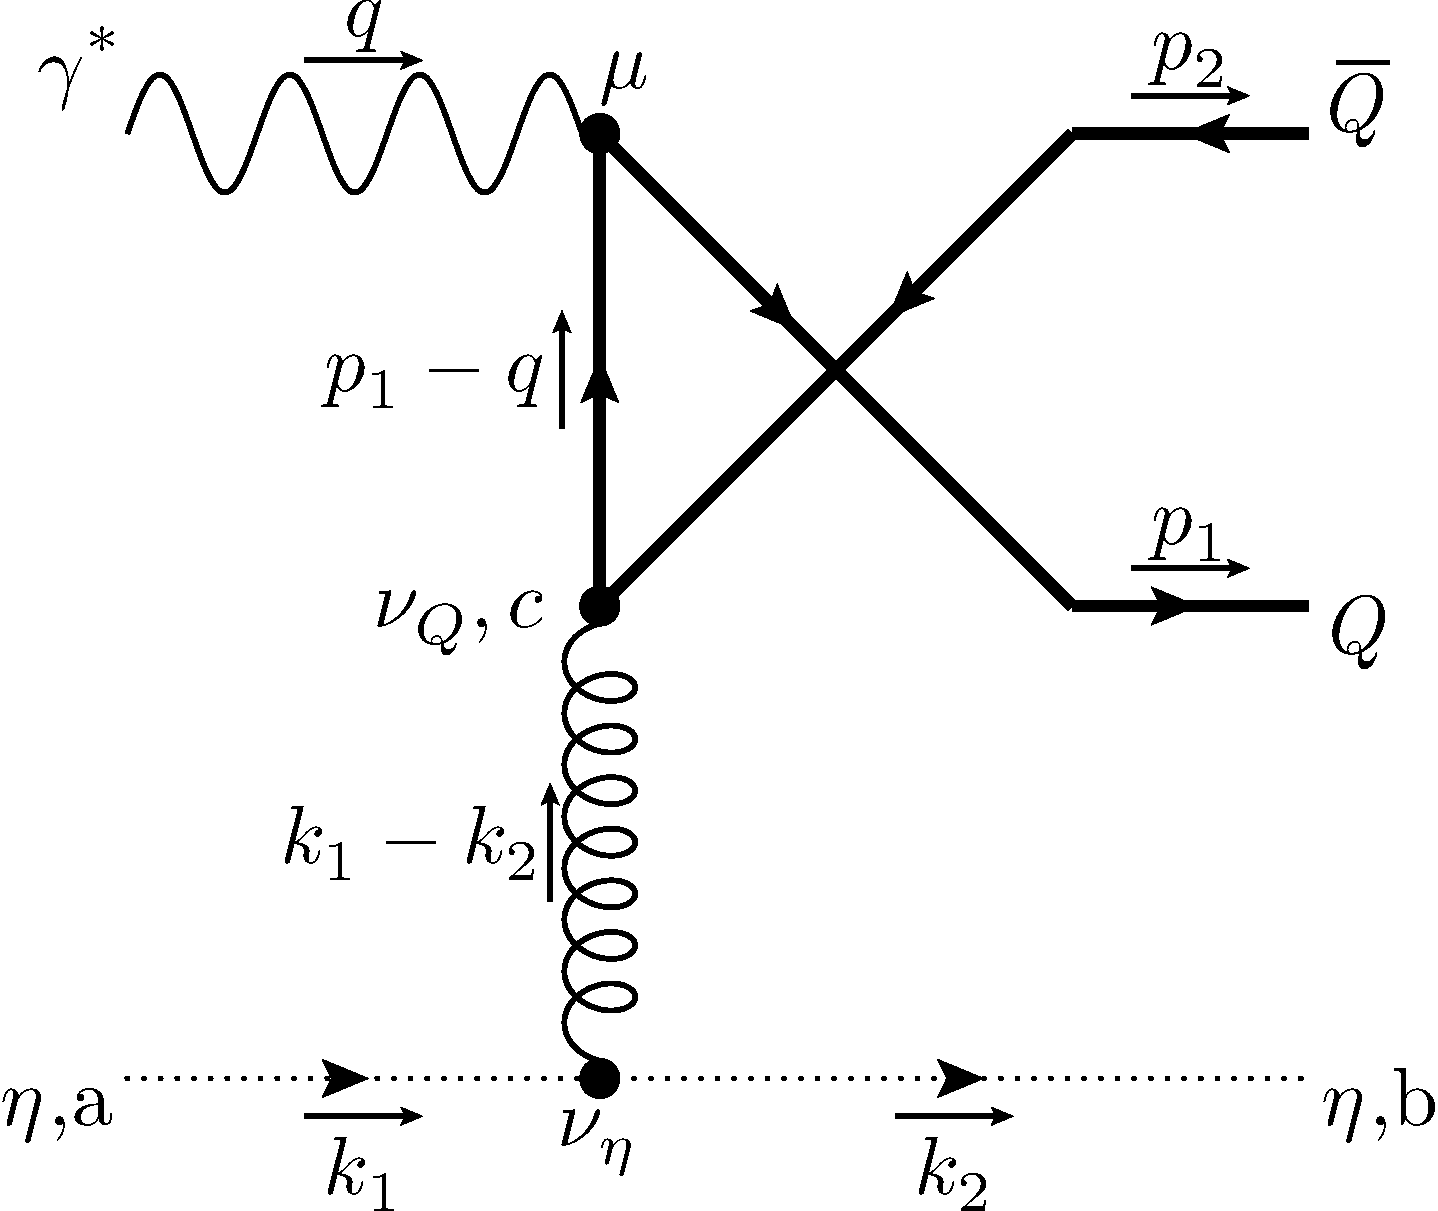
\includegraphics[width=\textwidth]{pyfeyn/nlo-gh-2}
		\caption{$i\Md^{(NLO,\Pgh)}_{2,\mu}$}
	\end{subfigure}\\
	\begin{subfigure}[t]{.42\textwidth}
		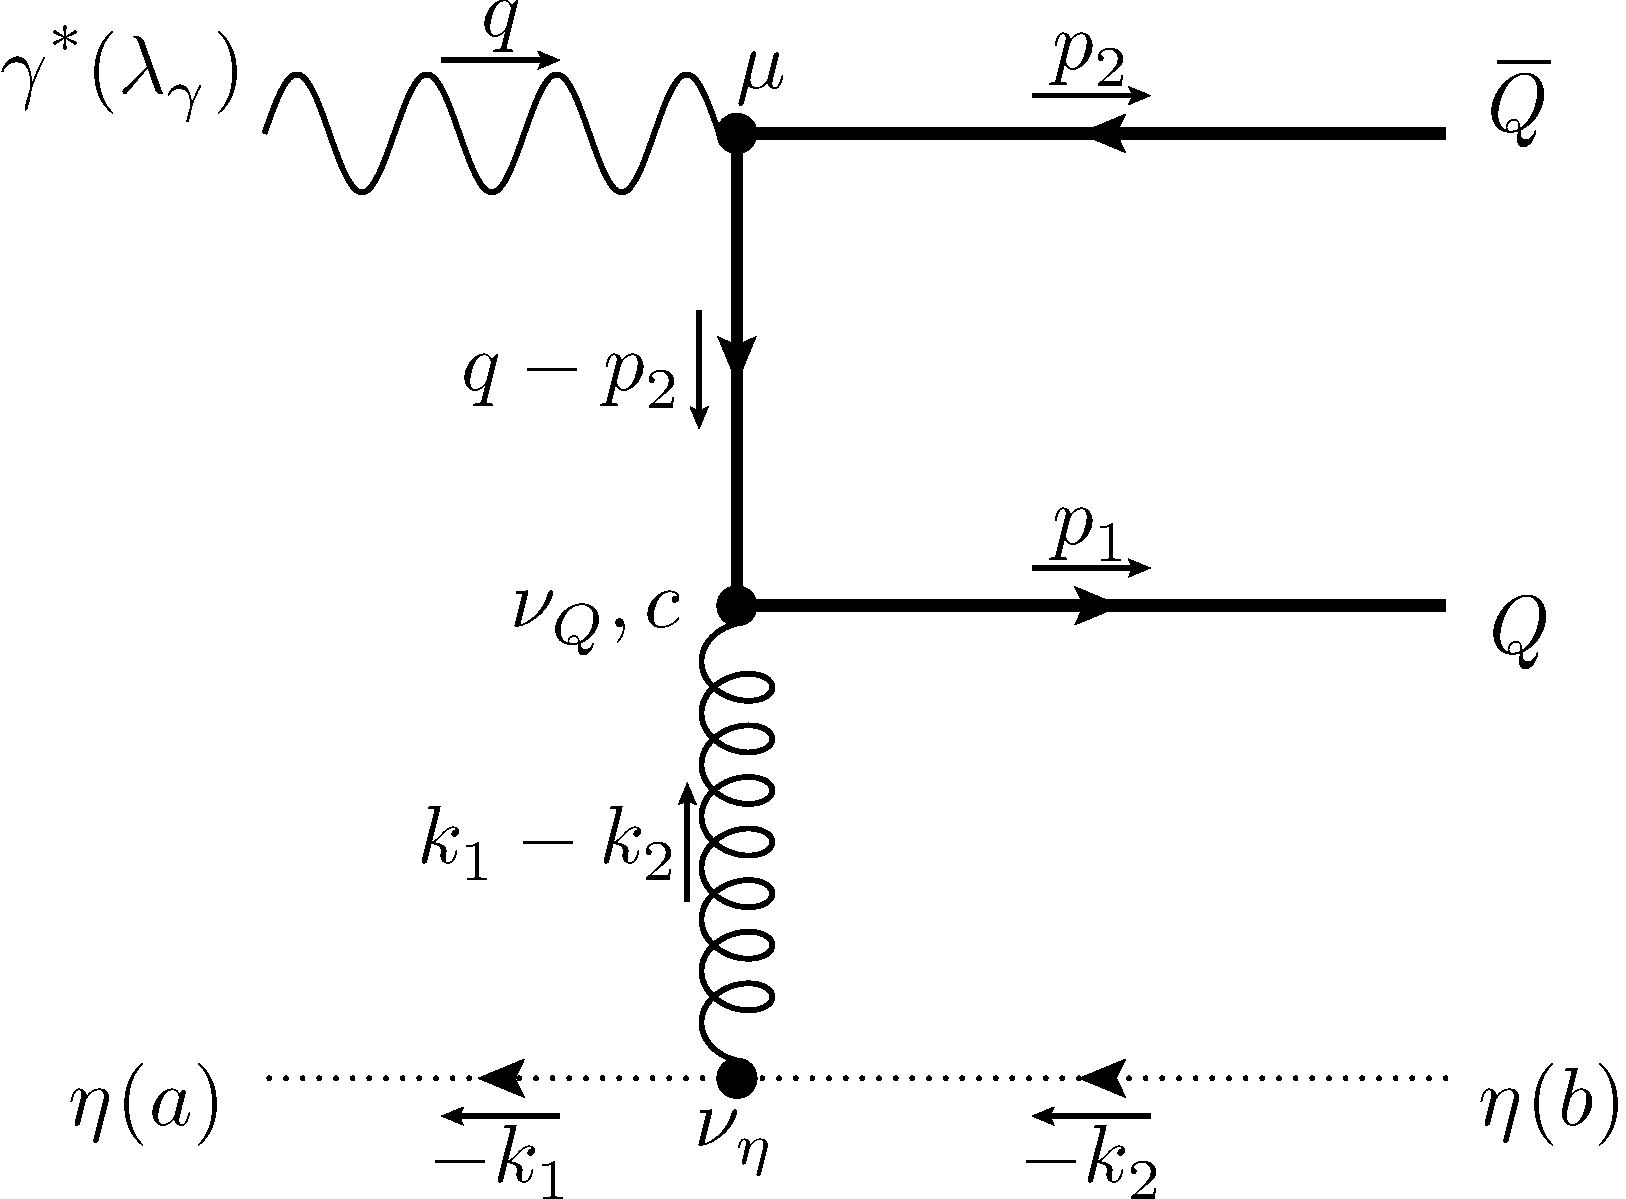
\includegraphics[width=\textwidth]{pyfeyn/nlo-gh-3}
		\caption{$i\Md^{(NLO,\Pgh)}_{3,\mu}$}
	\end{subfigure}\hspace{.1\textwidth}%
	\begin{subfigure}[t]{.42\textwidth}
		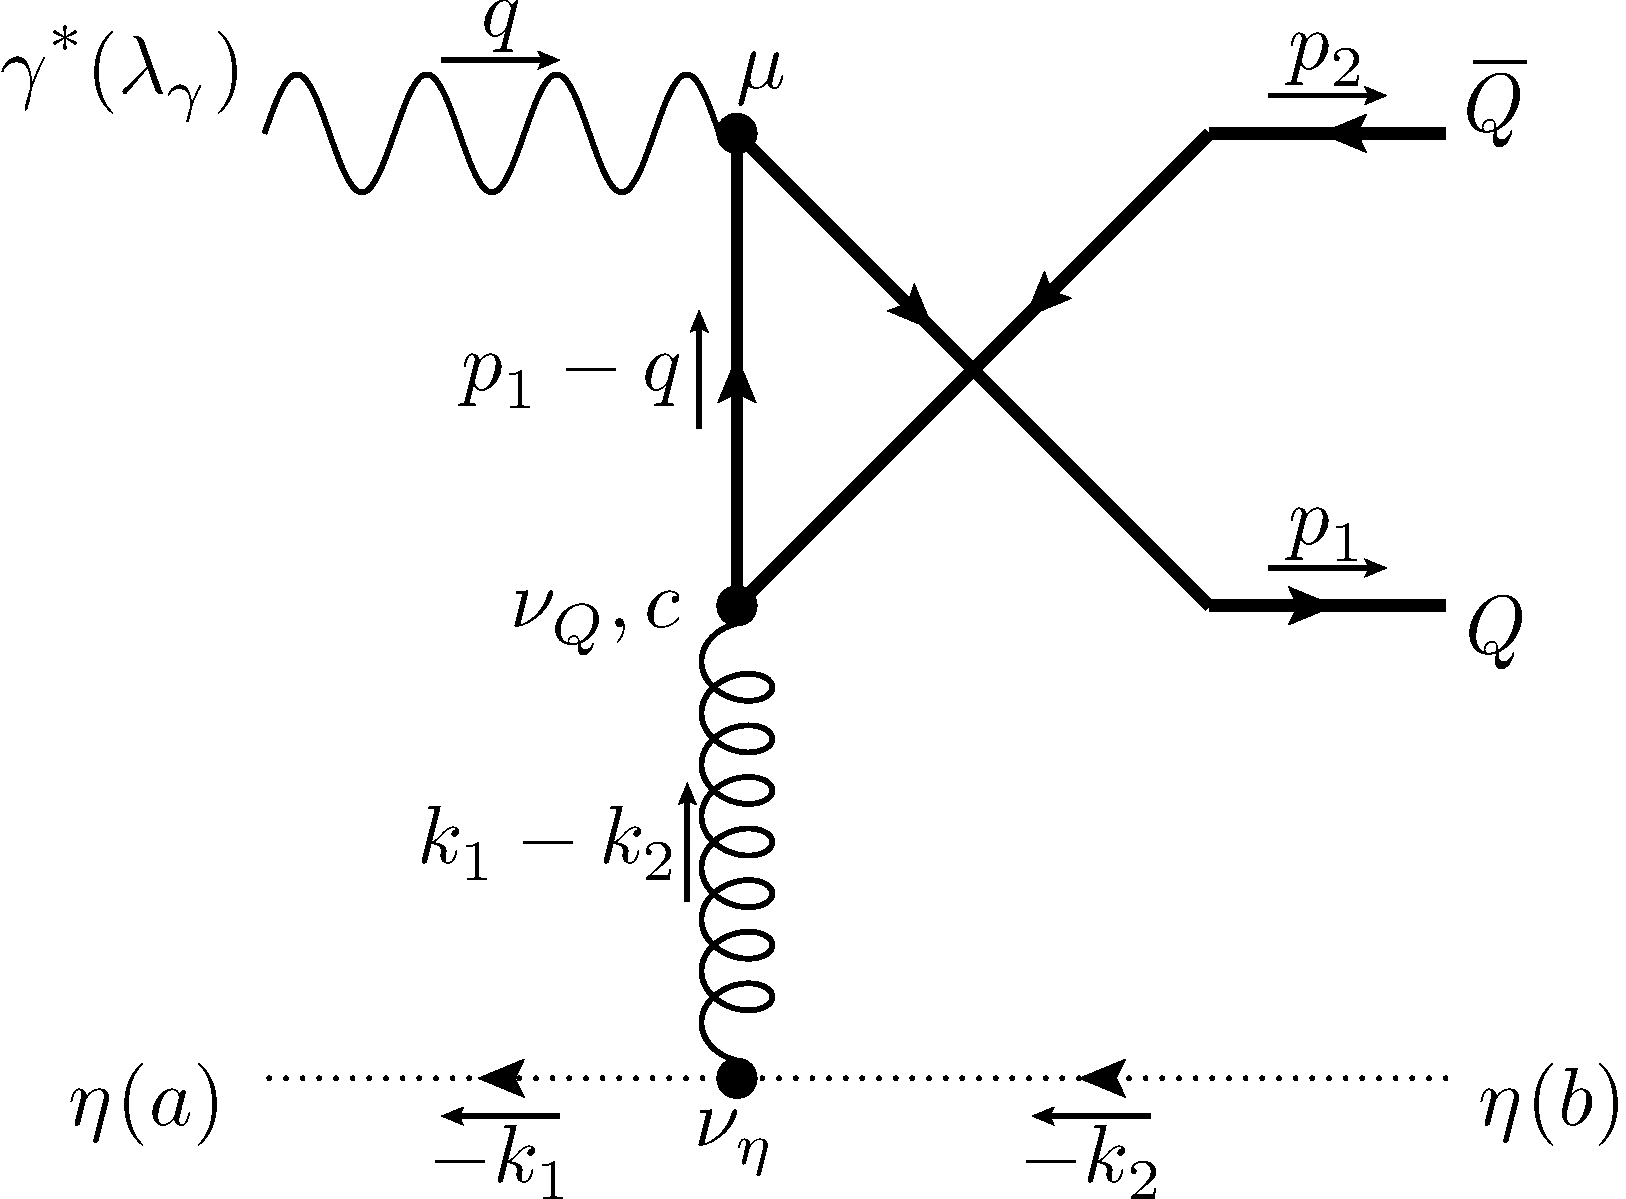
\includegraphics[width=\textwidth]{pyfeyn/nlo-gh-4}
		\caption{$i\Md^{(NLO,\Pgh)}_{4,\mu}$}
	\end{subfigure}
	\caption{NLO contributions by ghosts}\label{fig:FeynNLOgh}
\end{figure}

formula:
\begin{align}
i\Md^{(NLO,\Pgh)}_{1,\mu} &= \bar u(p_1)( igT_c\gamma^{\nu_Q})\frac{i(\slashed{q}-\slashed{p}_2+m)}{u_1}(-i e e_H \gamma_\mu) v(p_2)\cdot\frac{-ig_{\nu_Q,\nu_{\Pgh}}}{t'} \cdot (gf^{acb}k_2^{\nu_{\Pgh}})\\
i\Md^{(NLO,\Pgh)}_{2,\mu} &= \bar u(p_1)(-i e e_H \gamma_\mu) \frac{i(\slashed{p}_1-\slashed{q}+m)}{u_7}( igT_c\gamma^{\nu_Q})v(p_2)\cdot\frac{-ig_{\nu_Q,\nu_{\Pgh}}}{t'} \cdot (gf^{acb}k_2^{\nu_{\Pgh}})\\
i\Md^{(NLO,\Pgh)}_{3,\mu} &= \bar u(p_1)( igT_c\gamma^{\nu_Q})\frac{i(\slashed{q}-\slashed{p}_2+m)}{u_1}(-i e e_H \gamma_\mu) v(p_2)\cdot\frac{-ig_{\nu_Q,\nu_{\Pgh}}}{t'} \cdot (gf^{cab}(-k_1)^{\nu_{\Pgh}})\\
i\Md^{(NLO,\Pgh)}_{4,\mu} &= \bar u(p_1)(-i e e_H \gamma_\mu) \frac{i(\slashed{p}_1-\slashed{q}+m)}{u_7}(igT_c\gamma^{\nu_Q})v(p_2)\cdot\frac{-ig_{\nu_Q,\nu_{\Pgh}}}{t'} \cdot (gf^{cab}(-k_1)^{\nu_{\Pgh}})
\end{align}

color space:
\begin{align}
\abs{\Md^{(NLO,\Pgh)}_{1,\mu}+\Md^{(NLO,\Pgh)}_{2,\mu}}^2 &\sim f_{acb}f_{adb}\tr(T_cT_d) = N_C C_F C_A\\
\abs{\Md^{(NLO,\Pgh)}_{3,\mu}+\Md^{(NLO,\Pgh)}_{4,\mu}}^2 &\sim f_{cab}f_{dab}\tr(T_c T_d) = f_{acb}f_{adb}\tr(T_cT_d) = N_C C_F C_A
\end{align}
